\section{Les classes}

Les diagrammes de classes de l'architecture du logiciel ont été réalisés à l'aide des logiciel \emph{Architexa} et \emph{UML Lab} intégrés à \emph{Eclipse}. Nous ne parlerons donc que de notre architecture finale, obtenue au fur et à mesure des sprints et refactorings.

Étant donné l'étendue de l'application, nous ne pouvons pas présenter de diagramme UML à la fois complet et lisible dans ce rapport. Commençons donc par obtenir une vue d'ensemble du logiciel à l'aide du diagramme en couches visible en figure \vref{layered-packages}. En bleu, les packages de transformation des données. En vert, les packages utilitaires. En rouge, le cœur de l'application, qui inclue dans des sous-packages le modèle des données, la gestion de cache et les classes d'interface graphique. Les flèches, plus ou moins épaisses, indiquent une dépendance plus ou moins forte d'un package à un autre.
On remarque bien que le package diams constitue le cœur de l'application.
Les packages utilitaires peuvent être changés sans problèmes car ils ne dépendant pas d'autres packages.
Le package pixelmed constitue une bibliothèque de traitement de fichiers Dicom dont le cœur d'application dépend.
L'enjeu majeur a donc été de rendre l'architecture du cœur d'application la plus flexible possible pour limiter
l'effort requis en cas de changement de bibliothèques.


\begin{figure}[h]
\begin{center}
    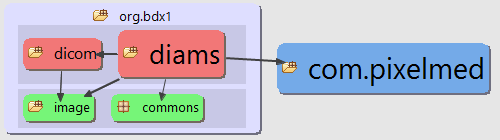
\includegraphics[width=11cm]{diagramme-couche}
\end{center}
    \caption{Diagramme en couches de l'application}
    \label{layered-packages}
\end{figure}

\subsection{Le modèle d'examen}

Voyons maintenant le diagramme des classes du modèle, en figure \vref{classes-model}.
En bleu, les classes utilitaires, en vert le modèle qui représente un examen et les données associées, et en
orange les éléments qui permettent de faire le lien entre le modèle et la bibliothèque d'extraction des images \emph{Pixelmed}.

La classe \verb+DefaultModelFactory+ permet d'interagir depuis l'extérieur avec le modèle d'un examen sans dépendre des autres classes.
La classe \verb+Examen+ est le composant principal qui permet de gérer les autres éléments du modèle.
Un ensemble d'interfaces permet de faciliter des modifications ultérieures sur le modèle.

Notez que la classe orange \verb+LisaImageAdapter+ est le seul élément de dépendance avec la bibliothèque externe \emph{Pixelmed}. Nous avons donc minimisé l'impact que peut créer le passage de \emph{Pixelmed} à un autre outil.


\begin{figure}[h]
\begin{center}
    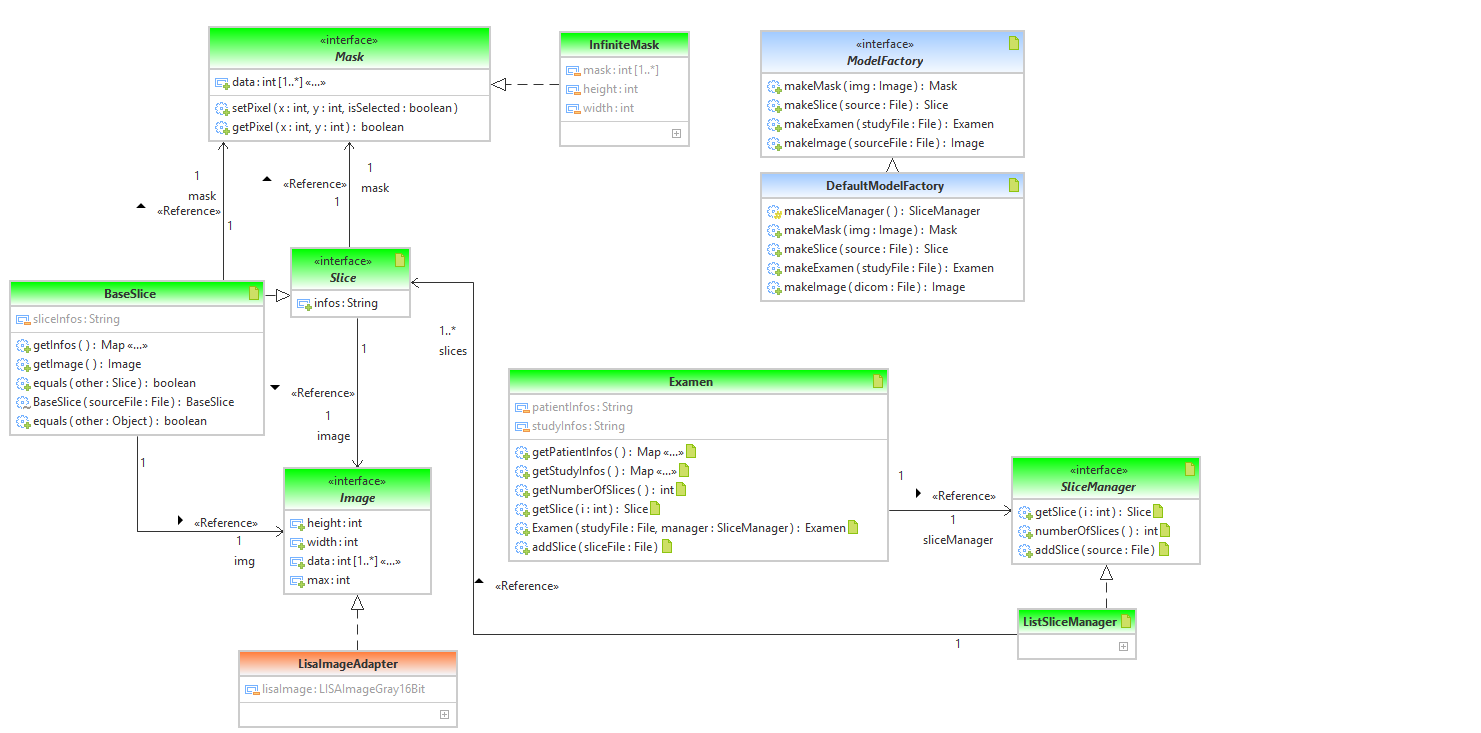
\includegraphics[width=11cm]{diagramme-classes-model}
\end{center}
    \caption{Diagramme de classes du modèle de l'application}
    \label{classes-model}
\end{figure}

\subsection{L'interface graphique}

Nous nous intéressons maintenant au diagramme des classes simplifié de la partie graphique, visible en figure \vref{classes-diams}. En bleu, les classes d'interface graphique. En orange, les classes d'interaction avec les fichiers et en vert la classe d'interaction avec le modèle.

La classe \verb+FileBrowserActivity+ permet, à l'ouverture de l'application, de sélectionner et d'ouvrir un examen parmi une arborescence de fichiers. Les classes \verb+ImageActivity+ et \verb+InfoDisplayActivity+ permettent de visualiser les composants de l'examen choisi et d'interagir avec.
La classe \verb+DicomDirFileHandler+ gère les traitements des fichiers lors de la navigation dans l'arborescence des fichiers.

On note que les dépendances entre l'interface graphique et les données sont limitées à deux classes. Nous avons minimisé l'impact d'un changement de bibliothèque d'interface graphique à ces deux classes.

\begin{figure}[h]
\begin{center}
    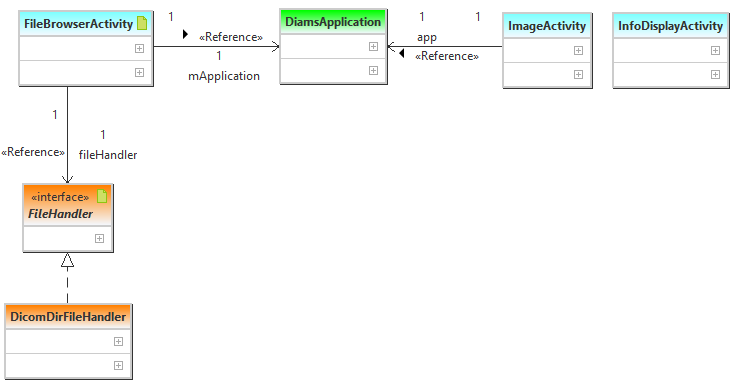
\includegraphics[width=11cm]{diagramme-classes-diams}
\end{center}
    \caption{Diagramme de classes de l'interface graphique de l'application}
    \label{classes-diams}
\end{figure}

\subsection{Système de cache}

Le développement d'une application mobile entraine des contraintes dues au materiel. La puissance du processeur et la quantité de mémoire vive sont limitées. Notre application devant gérer un grand nombre d'images, nous avons implémenté un système de cache afin de limiter l'occupation mémoire à un instant t, sans pour autant entraver les actions de l'utilisateur par de longs temps de chargement.

Afin que notre couche modèle puisse être réutilisée dans un contexte n'entrainant pas l'utilisation d'un cache, nous avons fait attention à séparer les classes responsables de ce cache des autres classes modèles. Cette problématique nous a tout d'abord conduit à séparer la gestion des coupes de l'Examen proprement dit à travers l'interface \verb+SliceManager+. Nous avons ensuite pu réaliser l'implémentation du cache indépendamment du modèle. La bibliothèque android contenant déjà un système de cache, nous avons décidé de l'utiliser pour implémenter \verb+SliceManager+. De cette façon, une seule classe de notre système de cache dépend d'android. Enfin, nous utilisons une nouvelle \verb+ModelFactory+ héritant de \verb+DefaultModelFactory+ afin de faire la liaison entre le modèle et le cache.

%insérer ici le diagramme
%voir commentaires supplémentaires en fonction du diagramme